\section{Task 4}
\FloatBarrier % Now figures cannot float above section title


\subsection{Simulink}

\begin{figure}[htbp]
    \centering
    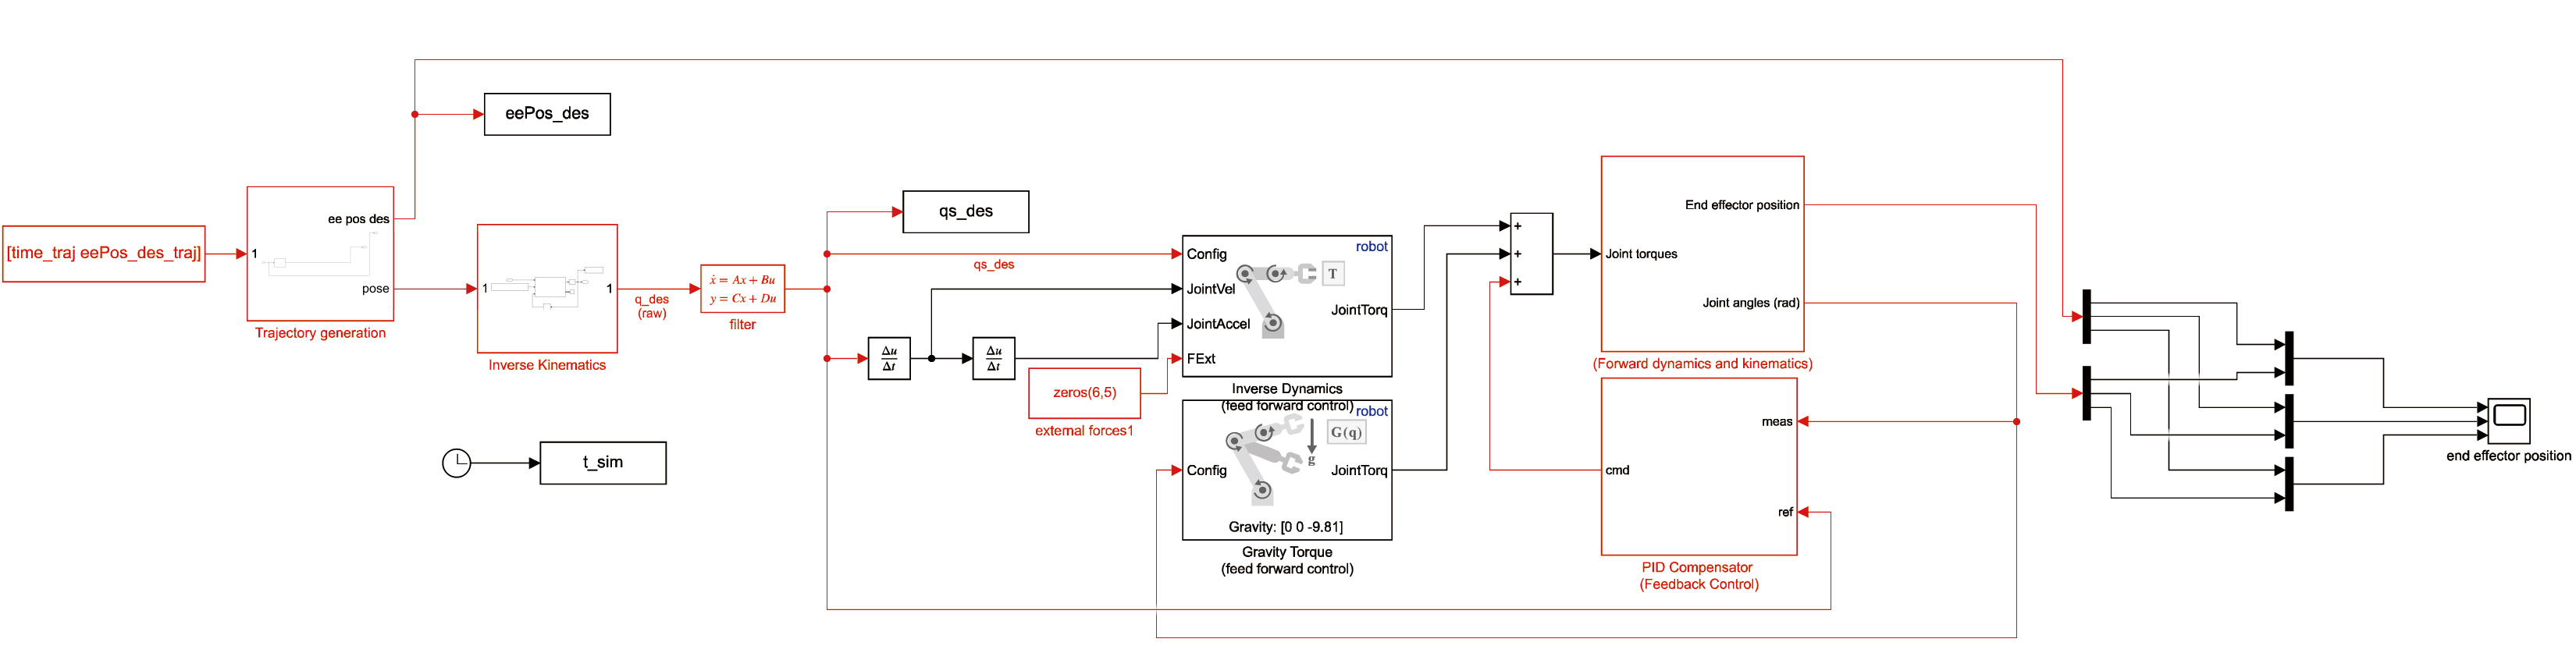
\includegraphics[width=17cm]{./fig/sim.jpg}
    \caption{plastic modules of rectangular section  }
    \label{f1}
\end{figure}

\subsubsection*{Tidy of the model}
To ensure aesthetic appeal, a modular design approach was adopted, where different modules represent different functionalities, thereby making the overall model's operation flow appear clear and concise.

\subsubsection*{Trajectory generation}

\begin{figure}[htbp]
    \centering
    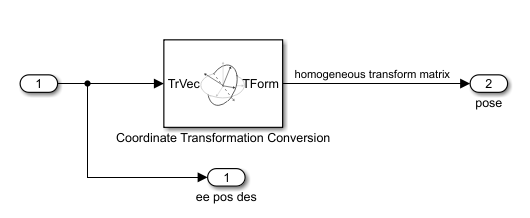
\includegraphics[width=8cm]{./fig/traj.png}
    \caption{plastic modules of rectangular section  }
    \label{f1}
\end{figure}

Trajectory generation module is an important component of robot motion planning, as it allows robots to move safely and efficiently in complex environments.This module is to convert signals from one coordinate system to another so that we can have easier control of the system. Additionally, the trajectory needs to be smooth, so that the robot does not make sudden changes in direction or speed that may destabilize the system or cause discomfort to human users.

We first calculate the path coordinate points and time series from the code, and use them as input parameters for trajectory calculation. Through trajectory calculation, we can obtain the expected end-effector position and the motion trajectory data applicable to each point after coordinate transformation (which is a 4001*3 data, recording the three-dimensional coordinate points of the path every 0.01 seconds and simulated for a total of 40 seconds).


\subsection{PID design}

\begin{figure}[htbp]
    \centering
    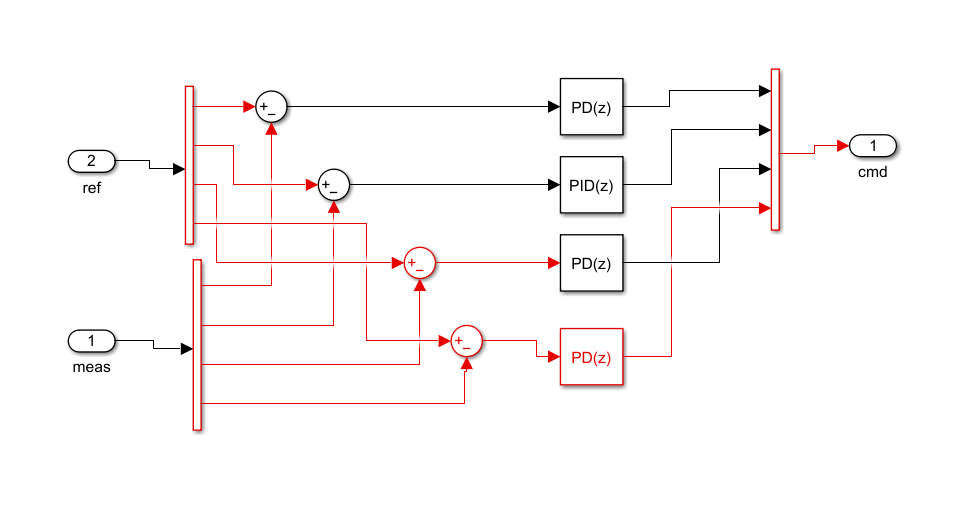
\includegraphics[width=10cm]{./fig/PID.png}
    \caption{plastic modules of rectangular section}
    \label{f1}
\end{figure}


With the aim of having better accruacy of the end effect position, we add a feedback control module. Feedback control is a control technique used in engineering to control a system by adjusting its behavior based on measured output signals. In feedback control, the output of the system is measured and compared to a desired end effect position. The difference between the measured output and the desired end effect position is called the error signal, which is then used to adjust the system's behavior through a feedback loop.

In the PID control module, we subtract the desired data from the actual data to obtain the error value, which is then used for PID calculation. We noticed that joints 1, 3, and 4 only use PD controllers because these three joints require a fast response speed and low overshoot, and have lower requirements for steady-state error. For joint 2, which uses a PID controller, it is sensitive to steady-state error due to its rotation around the y-axis. Although there may be difficulty in tuning, we successfully completed the debugging process.


\subsection{Results}

\begin{figure}[htbp]
    \centering
    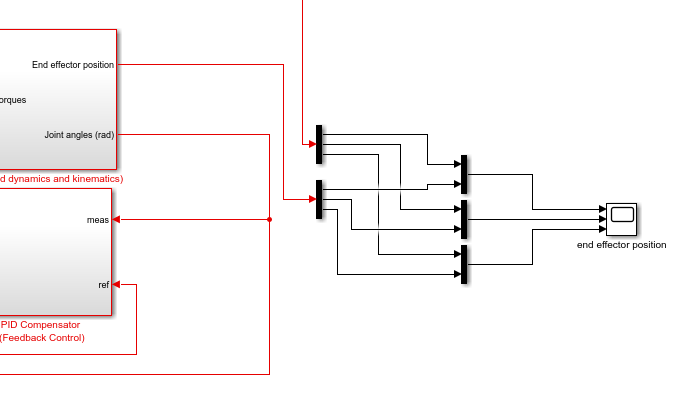
\includegraphics[width=7cm]{./fig/re.png}
    \caption{plastic modules of rectangular section}
    \label{f1}
\end{figure}

Finally, set the end effector positions and the desired end effector positoins as the input, draw the plot with their x y z positions followed by the time respectively.

\subsubsection*{Input torque}

\begin{figure}[htbp]
    \centering
    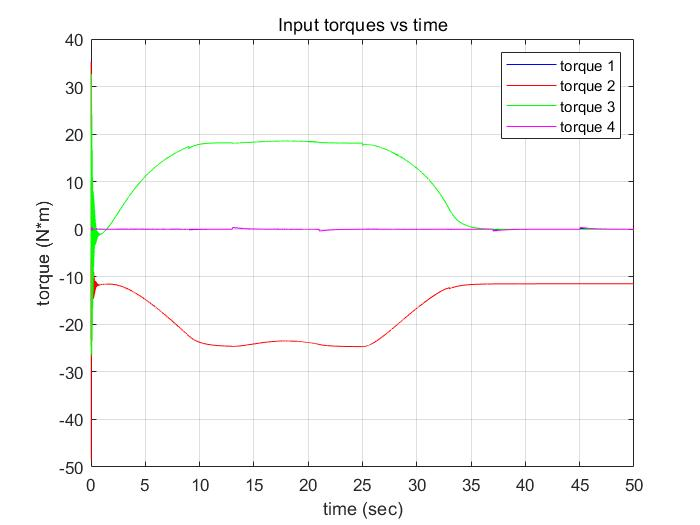
\includegraphics[width=10cm]{./fig/3.jpg}
    \caption{plastic modules of rectangular section}
    \label{f1}
\end{figure}


\subsubsection*{Joint angle}

\begin{figure}[htbp]
    \centering
    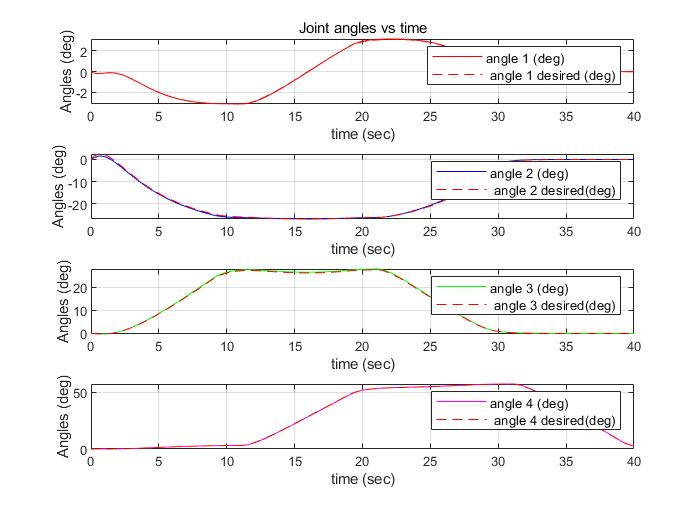
\includegraphics[width=8cm]{./fig/4.jpg}
    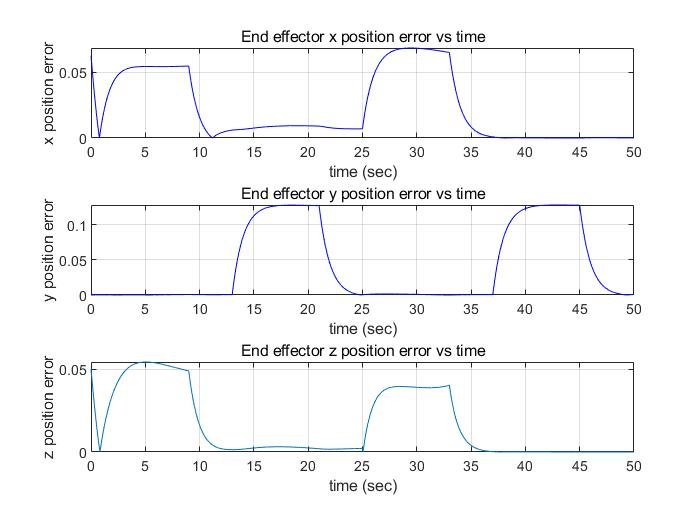
\includegraphics[width=8cm]{./fig/6.jpg}
    \caption{plastic modules of rectangular section}
    \label{f1}
\end{figure}

As we can see in the 'joint angle error' plot, 
The error of joint1 angle does not exceed the limit of $10^{-3}$, but it fluctuates throughout the process;
The error of joint2 angle is the largest, and it nearly reaches 0.02, the error tends to be stable except for large fluctuations at the peak throughout the process;
Both the maximum error of joint3 angle and joint4 angle are below 5*10-3, but joint3 angle error are steady increase to the maximum error, and remain stable on the maximum angle error; as for joint4 angle, there is almost no error in the first ten seconds, and there is always a period of stability after the changes of the error.
Overall, the errors are small and will not have a significant impact on the operation of the robot.




\subsubsection*{End Effector Position}

\begin{figure}[htbp]
    \centering
    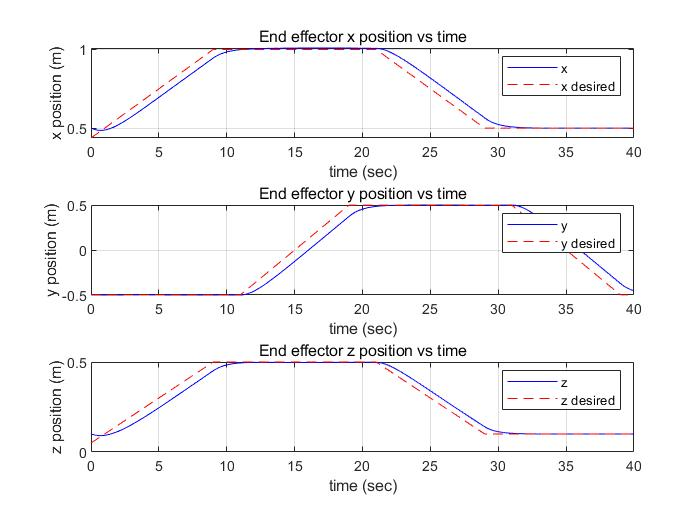
\includegraphics[width=8cm]{./fig/5.jpg}
    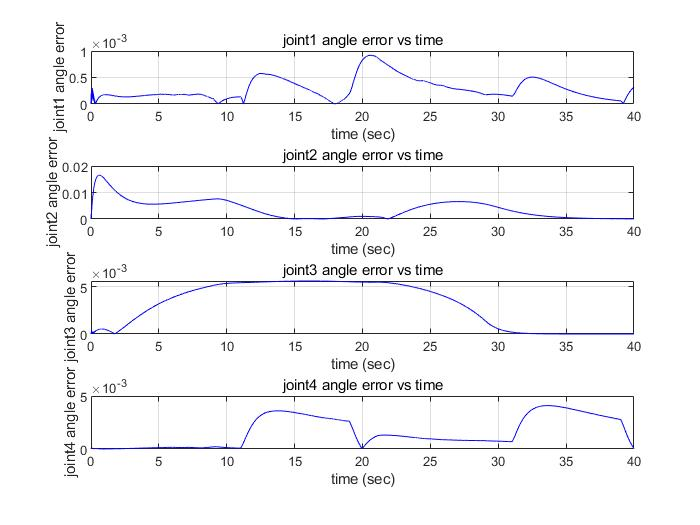
\includegraphics[width=8cm]{./fig/7.jpg}
    \caption{plastic modules of rectangular section}
    \label{f1}
\end{figure}

As we can see in the 'end effector position error' plot, the maximum error in end effector position on the x and z axes is below 0.05, while the maximum error on the y axis is slightly over 0.10. The errors in the x and z axes fluctuate simultaneously, while the error in the y axis gradually increases as the errors in the former axes begin to decrease. There is a small amount of error throughout the entire process, but it is not significant. It has almost no impact in reality.